\noindent Für die Analyse wurde die Python Bibliothek \glqq{}libpff\grqq{} in Version 20211114 verwendet. Diese Bibliothek wurde speziell für den Zugriff auf das Personal Folder File (PFF) und das Offline Folder File (OFF) entwickelt. Diese Formate werden von Microsoft Outlook verwendet, um E-Mail, Kontakte und andere Daten zu speichern. PFF und OFF werden dabei in mehreren Dateitypen verwendet, unter anderem auch bei PST \cite{GitHub.26.06.2022}. \smallskip

\noindent Zuerst wurden die PST-Dateien mithilfe von des Moduls pypff der Bibliothek libpff geöffnet (siehe Abb. \ref{fig:fileopen}). Im nächsten Schritt habe ich eine rekursive Funktion mit dem Namen parse\_folder definiert. Diese durchläuft die Ordner der .pst-Datei und zählt dabei die enthaltenen E-Mails in den jeweiligen Ordnern, zu sehen in Abbildung \ref{fig:pstfileaufbau}, wo der Ordner Unbekannt 4102 E-Mails enthält. Des Weiteren erzeugt die Funktion eine Print-Ausgabe auf der Konsole (siehe Abbildung \ref{fig:pstfileaufbau}), um den Aufbau der Ordnerstruktur eines .pst-Files zu sehen. \smallskip

\begin{figure}[!ht]
    \centering
    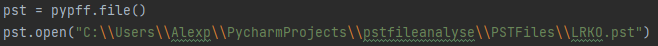
\includegraphics[width=0.75\textwidth]{images/File_open_libpff.PNG}
    \caption{Python Code - Öffnen der .pst-Datei mithilfe von libpff} 
    \label{fig:fileopen}
\end{figure}

\begin{figure}[!ht]
    \centering
    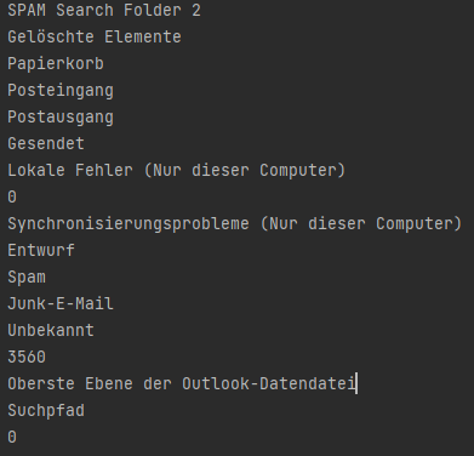
\includegraphics[width=0.50\textwidth]{images/PST_File_Aufbau_Python.png}
    \caption{Print Ausgabe - Aufbau der .pst-Datei} 
    \label{fig:pstfileaufbau}
\end{figure}


\noindent Die wichtigste Aufgabe der Funktion besteht jedoch darin, eine Liste mit den gewünschten Eigenschaften der E-Mails zu erstellen. In diesem Fall wurden von mir die Eigenschaften \glqq{}subject\grqq{}, \glqq{}sender\grqq{}, \glqq{}datetime\grqq{} und \glqq{}text\grqq{} ausgewählt. Der Aufbau dieser Funktion sowie die darin aufgeführten Eigenschaften der E-Mail sind in Abbildung \ref{fig:extraction} abgebildet. Nach der Funktionsdefinition wird die Funktion, wie in Abbildung \ref{fig:dataframeparstetocsv} zu sehen ist, aufgerufen. Die somit entstehende Liste \glqq{}messages\grqq{} wird anschließend mithilfe der Bibliothek pandas in einen DataFrame umgewandelt und dann in eine .CSV-Datei mit dem Namen \glqq{}MessagesPD.csv\grqq{} exportiert, um für die nachfolgende Weiterverarbeitung in einem geeigneterem Format bereitzuliegen. Abschließend ist hierbei noch zu erwähnen, dass die hier definierte Funktion relativ langsam ist und bei größeren Datensätzen eventuell optimiert werden müsste. Zur besseren Weiterverarbeitung der Daten wurden aus der großen .csv-Datei \glqq{}MessagesPD.csv\grqq{} mehrere .csv-Dateien erstellt. Der Beispielcode hierfür ist in Abbildung \ref{fig:csvseparation} zu sehen.


\begin{figure}[!ht]
    \centering
    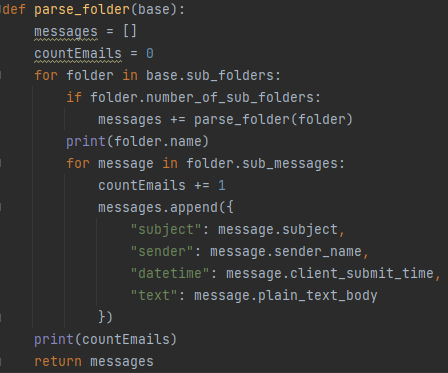
\includegraphics[width=0.75\textwidth]{images/Extraktion_aus_Pst_file.PNG}
    \caption{Python Code - Extraktion der Eigenschaften aus .pst-Datei} 
    \label{fig:extraction}
\end{figure}